% Section 7 -- Obfuscation. Diagnosed only: nothing here is repaired, and no sentence may imply otherwise.
% All numbers from the Phase 2 results files via paper/tools/gen_tables.py.
\section{Obfuscation}
\label{sec:obfuscation}

A claim that recurs in the activation-probing literature is that internal representations see through surface
transformations of the input: because the model must decode an obfuscated instruction in order to act on it, its
activations should carry the decoded meaning, and a probe reading them should be robust where a text classifier is
not. The claim is attractive and, on the models studied here, false. This section reports the anatomy of that failure.
Nothing in it is repaired; unlike Sections~\ref{sec:template} and~\ref{sec:read}, this is a diagnosis with no fix.

The study uses Gemma-2-9B and the $1{,}200$-prompt AILuminate hazard set under four conditions: plain text, Base64,
ROT13, and leetspeak. The design choice that makes it informative is the control: harmful prompts are scored against
benign prompts carrying \emph{the same} encoding. Without that control, a probe that has merely learned to recognise
Base64 reports excellent detection, and this turns out to be exactly what happens in the literature's favourable
results (Section~\ref{sec:circularity}).

\subsection{The model can decode; the probe cannot read the decoding}
\label{sec:decode}

The premise is testable directly: ask the model to decode the encoded prompt and grade what comes back.

% GENERATED by paper/tools/gen_tables.py -- do not edit by hand.
% sources: results/phase2/p1_decode.json
\begin{table}[!t]
\caption{Behavioural decode test on Gemma-2-9B: can the model recover the plaintext of an encoded prompt when
asked to? Grades are exact (normalised string match), partial (similarity $\geq 0.6$ or $\geq 60\,\%$ word
cover) and fail. No reply in either condition was a refusal, so these grades measure decoding ability rather
than safety behaviour.}
\label{tab:decode}
\centering
\setlength{\tabcolsep}{3.5pt}
\footnotesize
\begin{tabular}{lcccccc}
\toprule
Encoding & $n$ & exact & partial & fail & refusals & mean similarity \\
\midrule
base64 & 20 & 6 & 14 & 0 & 0 & 0.98 \\
rot13 & 20 & 0 & 0 & 20 & 0 & 0.24 \\
\bottomrule
\end{tabular}
\end{table}

Table~\ref{tab:decode} shows the two encodings behave completely differently. Base64 is recovered in all $20$ cases,
$6$ of them verbatim, at a mean similarity of $0.98$ to the plaintext; the misses are single-word slips. ROT13 is not
recovered at all: the model produces unrelated filler, and mean similarity is $0.24$. No reply in either condition was
a refusal, so this measures decoding ability rather than safety behaviour.

This bounds where a decoded representation could be looked for. Base64 is the condition in which the model
demonstrably forms the decoding, so it is the condition in which a decoded representation could exist to be read;
ROT13 is not, because the model never forms the decoding at all. Behavioural decoding does not by itself imply that
the decoded content is linearly recoverable at any particular position --- that is the question the sweep asks. The result also breaks the symmetry that makes ``obfuscation robustness'' sound like one property: a defence
can only inherit robustness from a capability the model actually has.

\subsection{No block, mode, or probe construction separates encoded harm}
\label{sec:sweep}

We swept every decoder block from $14$ to $35$ (roughly $33\,\%$ to $85\,\%$ depth), in both template modes, with two
probe constructions---the shipped direction and a direction retrained per block and per mode---and in both activation
spaces of Section~\ref{sec:tensor}. That is $176$ scored cells per space per encoding.

% GENERATED by paper/tools/gen_tables.py -- do not edit by hand.
% sources: results/phase2/p2_summary_mlp.json, results/phase2/p2_confounds.json
\begin{table}[!t]
\caption{Obfuscation sweep on Gemma-2-9B: the best AUC over $22$ blocks for each encoding, as
raw/length-stratified. Harmful prompts are scored against benign prompts carrying \emph{the same} encoding, so
a probe that merely detects the encoding gains nothing. Encoded columns collapse under the length control;
plain and leetspeak do not.}
\label{tab:obfuscation_sweep}
\centering
\setlength{\tabcolsep}{3pt}
\footnotesize
\begin{tabular}{llcccc}
\toprule
Probe & Mode & none & base64 & rot13 & leetspeak \\
\midrule
shipped & raw & 0.71/0.63 & 0.74/0.64 & 0.68/0.76 & 0.66/0.64 \\
shipped & templated & 0.86/0.83 & 0.83/0.66 & 0.83/0.72 & 0.75/0.76 \\
retrained & raw & 0.78/0.76 & 0.65/0.55 & 0.91/0.79 & 0.76/0.72 \\
retrained & templated & 0.84/0.86 & 0.91/0.64 & 0.85/0.74 & 0.73/0.78 \\
\bottomrule
\end{tabular}
\end{table}

Figure~\ref{fig:obfuscation} shows the sweep in full for the most favourable configuration.

\begin{figure*}[!t]
\centering
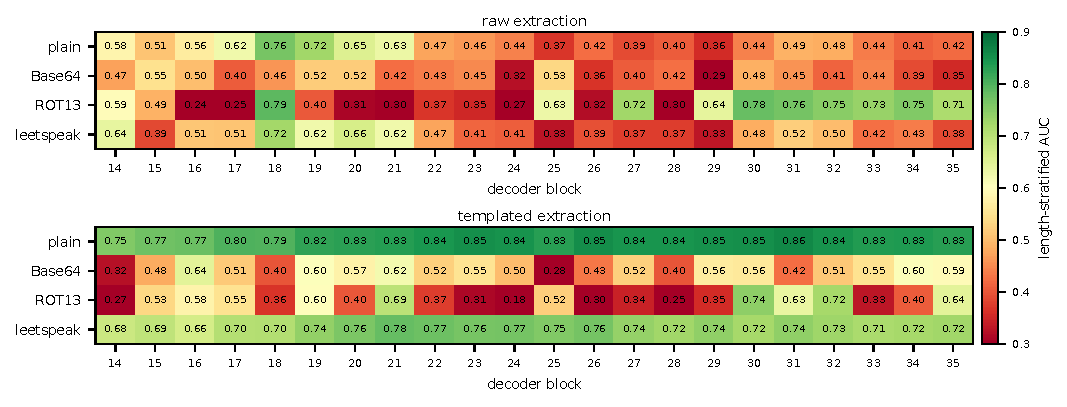
\includegraphics[width=\textwidth]{figures/fig_obfuscation}
\caption{No configuration separates encoded-harmful from encoded-benign prompts once prompt length is controlled.
Each cell is the length-stratified AUC at one decoder block, scoring harmful against benign prompts carrying the same
encoding. \textbf{The configuration shown is the best-performing one in the entire sweep}---the probe retrained per
block and per mode, read in the MLP-branch space the probes under study occupy---so what fails here is the strongest
case available, not a weak probe. Plain text and leetspeak
remain readable across the depth of the network; Base64 and ROT13 sit at or near chance everywhere, with a median of
$0.513$ over the $132$ encoded cells and a maximum of $0.787$. The uncontrolled versions of several of these cells
reach $0.85$--$0.92$, which is what length stratification removes.}
\label{fig:obfuscation}
\end{figure*}

Read the two numbers in each cell together. Several cells reach $0.85$--$0.92$ raw on Base64 and ROT13, which taken
alone would look like a positive result. In those same cells the probe score correlates with prompt length at
Spearman $\rho$ up to $+0.95$, and once length is stratified they fall to $0.49$--$0.65$. The best length-stratified
figure anywhere in the sweep is $0.73$ for Base64 and $0.79$ for ROT13, and the median across the $176$ cells is at or
below chance for both. Plain text and leetspeak lose almost nothing under the same control.

A second control settles the interpretation. If a block represented the decoded content of an encoded prompt, the
probe's score on the encoded prompt should track that same prompt's plain-text score at the same block. Across every
cell, that correlation is at most $0.36$ for Base64 and ROT13 and mostly below $0.2$, against $0.65$--$0.81$ for
leetspeak. Encoded-prompt scores carry essentially no information about what the prompt says.

Leetspeak is the exception that clarifies the rule. It leaves most characters readable, the probe treats it as noisy
plain text, and detection is nearly unchanged from plain ($46.5\,\%$ against $47.8\,\%$ at the shipped threshold). It
is not an obfuscation for this probe, and reporting it beside Base64 and ROT13 as though the three were comparable
overstates robustness considerably.

\subsection{How the favourable result is manufactured}
\label{sec:circularity}

The reason this matters is that a strong obfuscation result is easy to produce by accident.

% GENERATED by paper/tools/gen_tables.py -- do not edit by hand.
% sources: results/phase2/p3_circularity.json
\begin{table*}[!t]
\caption{Training-set circularity. Each cell reads detection / false-positive rate on \emph{equally encoded}
benign prompts / AUC. A probe whose training set contains encoded prompts reports near-perfect detection of
encoded harmful prompts while flagging just as many encoded benign ones, at below-chance AUC. Removing the
encoded prompts from training drops encoded detection to zero.}
\label{tab:circularity}
\centering
\setlength{\tabcolsep}{2pt}
\scriptsize
\begin{tabular}{llcccccccccccc}
\toprule
 & & \multicolumn{3}{c}{none} & \multicolumn{3}{c}{base64} & \multicolumn{3}{c}{rot13} & \multicolumn{3}{c}{leetspeak} \\
\cmidrule(lr){3-5} \cmidrule(lr){6-8} \cmidrule(lr){9-11} \cmidrule(lr){12-14}
Training set & Mode & det & FPR & AUC & det & FPR & AUC & det & FPR & AUC & det & FPR & AUC \\
\midrule
with encoded training prompts & raw & 0.99 & 0.72 & 0.90 & 1.00 & 1.00 & 0.29 & 1.00 & 1.00 & 0.29 & 1.00 & 1.00 & 0.77 \\
with encoded training prompts & templated & 0.77 & 0.31 & 0.82 & 1.00 & 1.00 & 0.26 & 1.00 & 1.00 & 0.04 & 0.89 & 0.73 & 0.71 \\
plain-only ablation & raw & 0.66 & 0.31 & 0.75 & 0.00 & 0.00 & 0.51 & 0.00 & 0.00 & 0.55 & 0.44 & 0.11 & 0.76 \\
plain-only ablation & templated & 0.71 & 0.19 & 0.82 & 0.00 & 0.00 & 0.53 & 0.00 & 0.00 & 0.29 & 0.74 & 0.42 & 0.72 \\
\bottomrule
\end{tabular}
\end{table*}

Table~\ref{tab:circularity} reconstructs a training recipe in which $30$ of the $81$ positive examples are themselves
encoded prompts. It reproduces the headline: essentially every Base64 and ROT13 harmful prompt is flagged. It also
flags essentially every Base64 and ROT13 \emph{benign} prompt, and the harmful-versus-benign AUC in those conditions
is $0.04$--$0.29$---below chance, because within the encoded prompts the longer ones, which are the harmful ones,
score \emph{lower}. The direction has learned ``is encoded'', not ``is harmful''. Remove the encoded examples from
training and encoded detection falls to zero.

An evaluation without an equally-encoded benign control cannot tell these two situations apart, and that control is
absent from the setups we are aware of. This is the same structure as the length confound in
Section~\ref{sec:controls}: a number that is real, reproducible, and measuring something other than the claim.

\subsection{What the probe adds over the model's own behaviour}
\label{sec:obf_refusal}

Finally, the refusal control. On plain text the probe's detections concentrate on prompts the model refuses anyway:
$81\,\%$ of refused harmful prompts are flagged against $22\,\%$ of answered ones, so the marginal value over the
model's existing behaviour is smaller than the headline detection rate suggests. Under Base64 and ROT13 the probe
detects nothing regardless of refusal---$0$ of $25$ sampled harmful prompts in both encodings---while the model itself
refuses $8$ of $25$ Base64 prompts, which it can decode, and $1$ of $25$ ROT13 prompts, which it cannot.

\subsection{What may and may not be claimed}
\label{sec:obf_claims}

Stated precisely, so that the negative result is not overread in either direction:

\begin{itemize}
\item Gemma-2-9B decodes Base64 in generation and does not decode ROT13.
\item Within the searched space --- $22$ blocks, two template modes, two probe constructions, two activation spaces,
      all at the last token --- no configuration separates Base64- or ROT13-encoded harmful prompts from equally
      encoded benign prompts once prompt length is controlled. The search did not vary read position, which
      Section~\ref{sec:read} shows can dominate everything else; that is the largest gap in this negative result.
\item Apparent successes on encoded prompts in this design are explained by prompt length, and reported successes
      elsewhere are explained by training on the encodings being tested, with no encoded benign control to expose it.
\item Leetspeak is read as noisy plain text and should not be grouped with the other two.
\end{itemize}

What this does \emph{not} establish is a general impossibility. We tested one model family at one scale, one probe
construction, and last-token reads. Section~\ref{sec:read} showed that a read position can matter more than anything
else in the setup, and we did not sweep read positions here. The honest summary is that the obfuscation-robustness
claim is unsupported on these models and that the experiments which appear to support it elsewhere have a control
missing---not that no representation of decoded content exists anywhere in any model.
